\documentclass{beamer}

\usepackage{inter}
\usepackage{url}
\usepackage[italian]{babel}
\usepackage{graphicx}
\usepackage{hyperref}
\usepackage{tikz}
\usepackage{fontawesome}

\hypersetup{
  pdfpagemode=FullScreen,
  colorlinks=true
}

\setbeamertemplate{navigation symbols}{} % remove navigation symbols

\title{Tabula}
\author{
  Alfredo Carlino \texttt{246025} \newline
  \and Giorgio Carlino \texttt{246038} \newline
  \and Mario G. D'Andrea \texttt{245940}}
\institute{Corso di Web Applications \\ C.d.S. Informatica $\cdot$ DeMaCs \\ Università della Calabria}
\titlegraphic{
\includegraphics[width=2cm]{unical}}
\date{Giugno 2025}

\begin{document}
\maketitle

\begin{frame}
  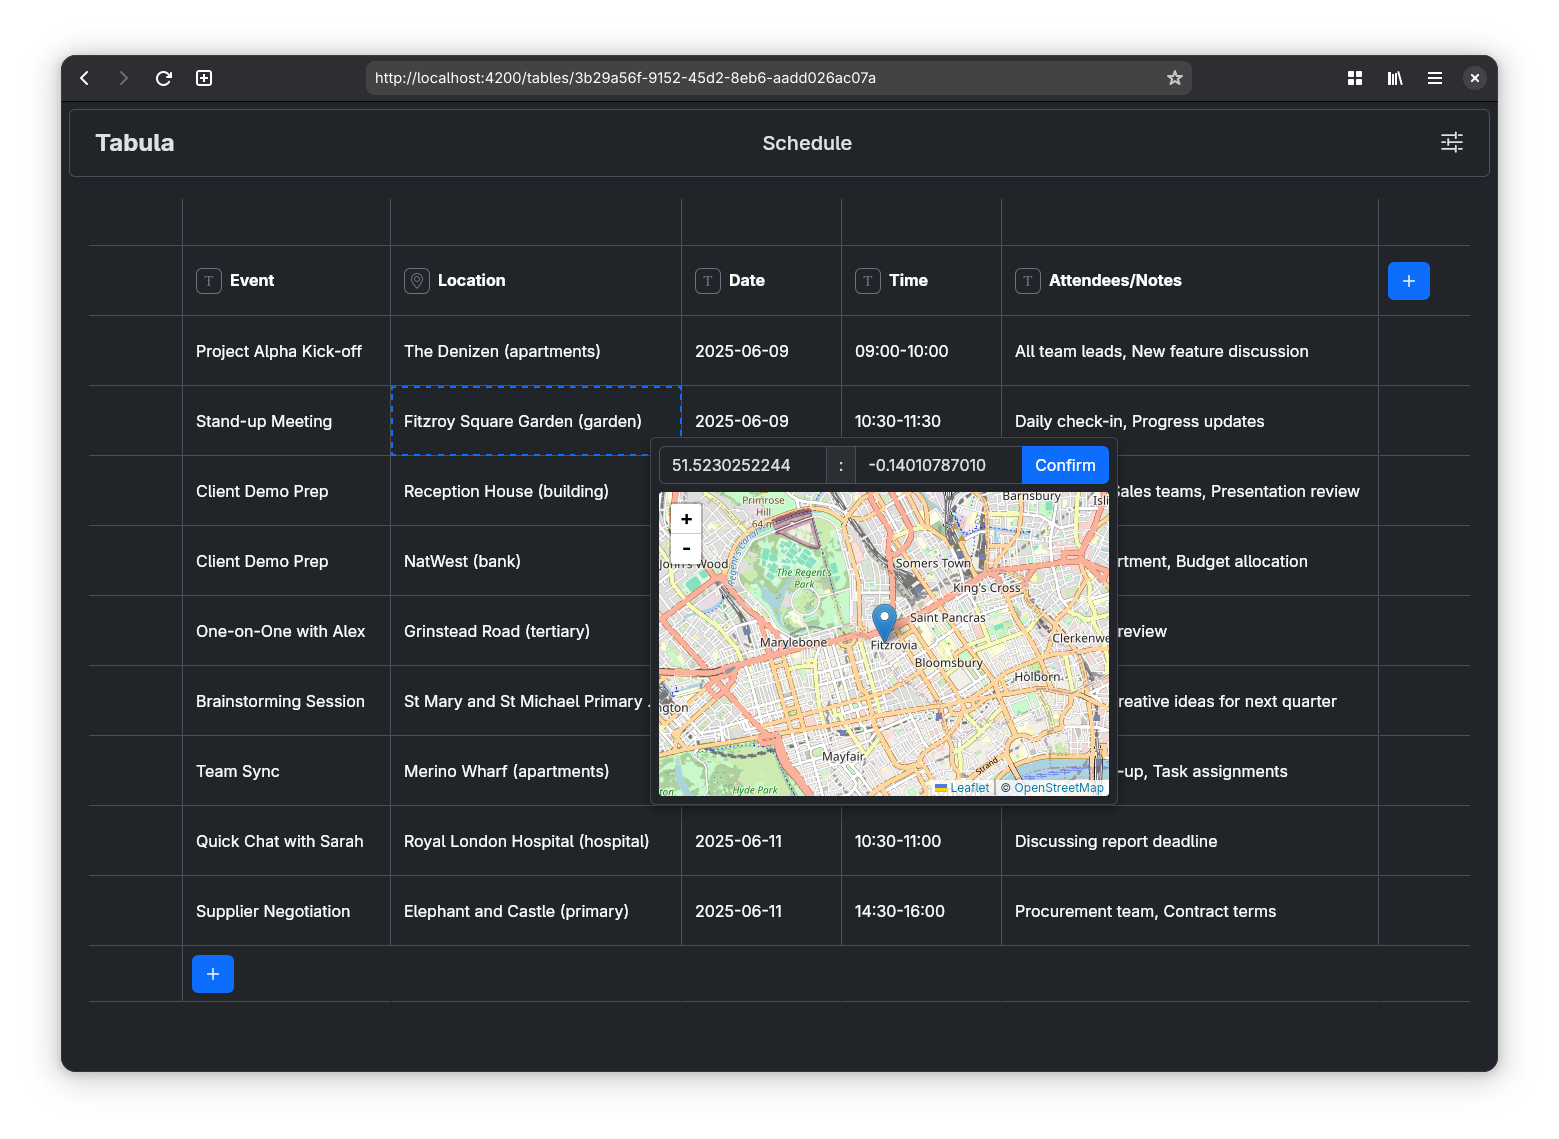
\includegraphics[width=\textwidth]{demo}
  \centering  \href{https://github.com/bytestrick/tabula}{\faGithub\ github.com/bytestrick/tabula}
\end{frame}

\begin{frame}
  \frametitle{Descrizione generale}

  Tabula consente di organizzare dati in formato tabellare facilitando l'accesso e la modifica. Piuttosto che un foglio di calcolo, si può considerare l'app come una base di dati con cui si può interagire direttamente.

  \vspace{10pt}

  Ogni tabella in Tabula è composta da diverse colonne, ognuna con un \textbf{tipo} assegnato: numero, testo, data, posizione geografica, somma monetaria, ecc.

  \vspace{10pt}

  La facilità di utilizzo delle tabelle le rende uno strumento perfetto per tenere traccia delle letture, sia concluse che pianificate; oppure raggruppare in un unico punto i task pianificati (to-do) e aggregarli in classi usando il tipo \textit{tag}, corredandoli di una data e una posizione geografica opzionalmente; o ancora tracciare la performance di una squadra di calcio, derivando informazioni statistiche dagli esiti delle singole partite.

\end{frame}

\begin{frame}
  \frametitle{Layout e schermate}

  L’applicazione si compone di tre schermate principali:

  \begin{itemize}
    \item[\faUser] \textbf{\textit{Sign Up} \& \textit{Sign In}} \hspace{3pt} Viene mostrata esclusivamente agli utenti non ancora registrati, permette la creazione di un account, necessario per accedere alla piattaforma.

Una volta completata la registrazione, l’utente viene automaticamente reindirizzato alla schermata di \textit{sign-in}, dove può autenticarsi utilizzando le credenziali appena fornite.

    \item[\faHome] \label{ui_home} \textbf{Home} \hspace{3pt} È punto di accesso principale dell’utente dopo l'accesso. Qui è possibile visualizzare un riepilogo di tutte le tabelle create, con la possibilità di aggiungerne di nuove. Ogni tabella elencata consente operazioni di modifica o eliminazione.

    \item[\faTable] \label{ui_table} \textbf{Table} \hspace{3pt} Dedicata alla modifica e gestione dei contenuti all'interno di una singola tabella.

  \end{itemize}
\end{frame}

\begin{frame}
  \frametitle{Navigazione tra schermate}

  La navigazione segue un \textbf{modello ad hub}, con il seguente flusso:

  \begin{enumerate}
    \item L’utente accede alla schermata principale (\hyperref[ui_home]{Home})
    \item Da qui può essere reindirizzato a pagine secondarie (es. \hyperref[ui_table]{Table}) per svolgere azioni
specifiche
    \item Una volta completata l’attività, viene riportato alla schermata principale
  \end{enumerate}

\end{frame}

\begin{frame}
  \frametitle{Account e Navbar}

  \begin{columns}
    \begin{column}{0.53\textwidth}
      Per rendere disponibili in qualsiasi momento le informazioni dell’account e delle impostazioni (come il tema dell’interfaccia), è presente una sidebar integrata nella navbar, accessibile da qualsiasi schermata.
    \end{column}
    \begin{column}{0.48\textwidth}
      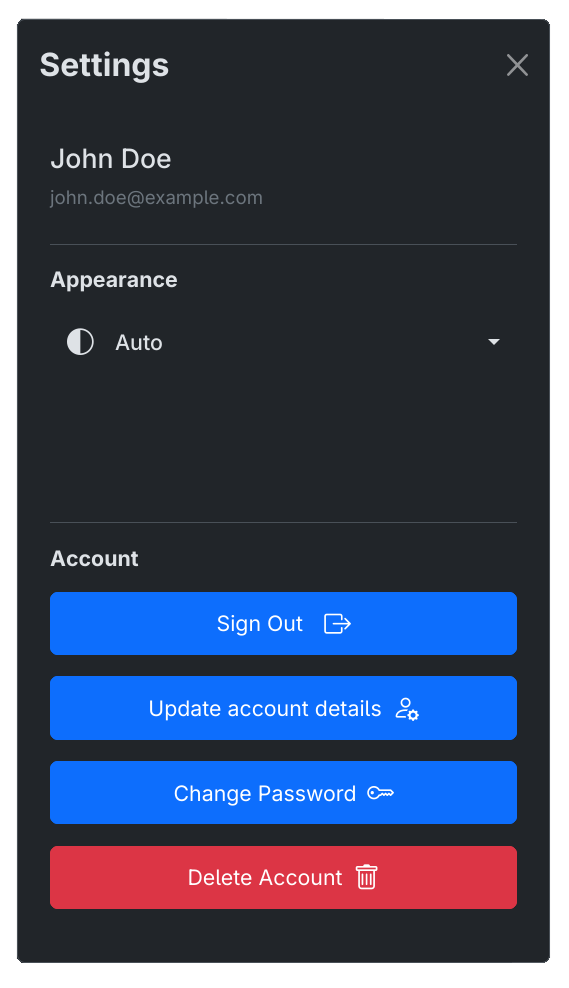
\includegraphics[width=5cm]{sidebar.png}
    \end{column}
  \end{columns}
\end{frame}

\begin{frame}
  \frametitle{Gerarchia visiva}

  L’interfaccia dell’applicazione è organizzata secondo una struttura a griglia.

  \begin{figure}
    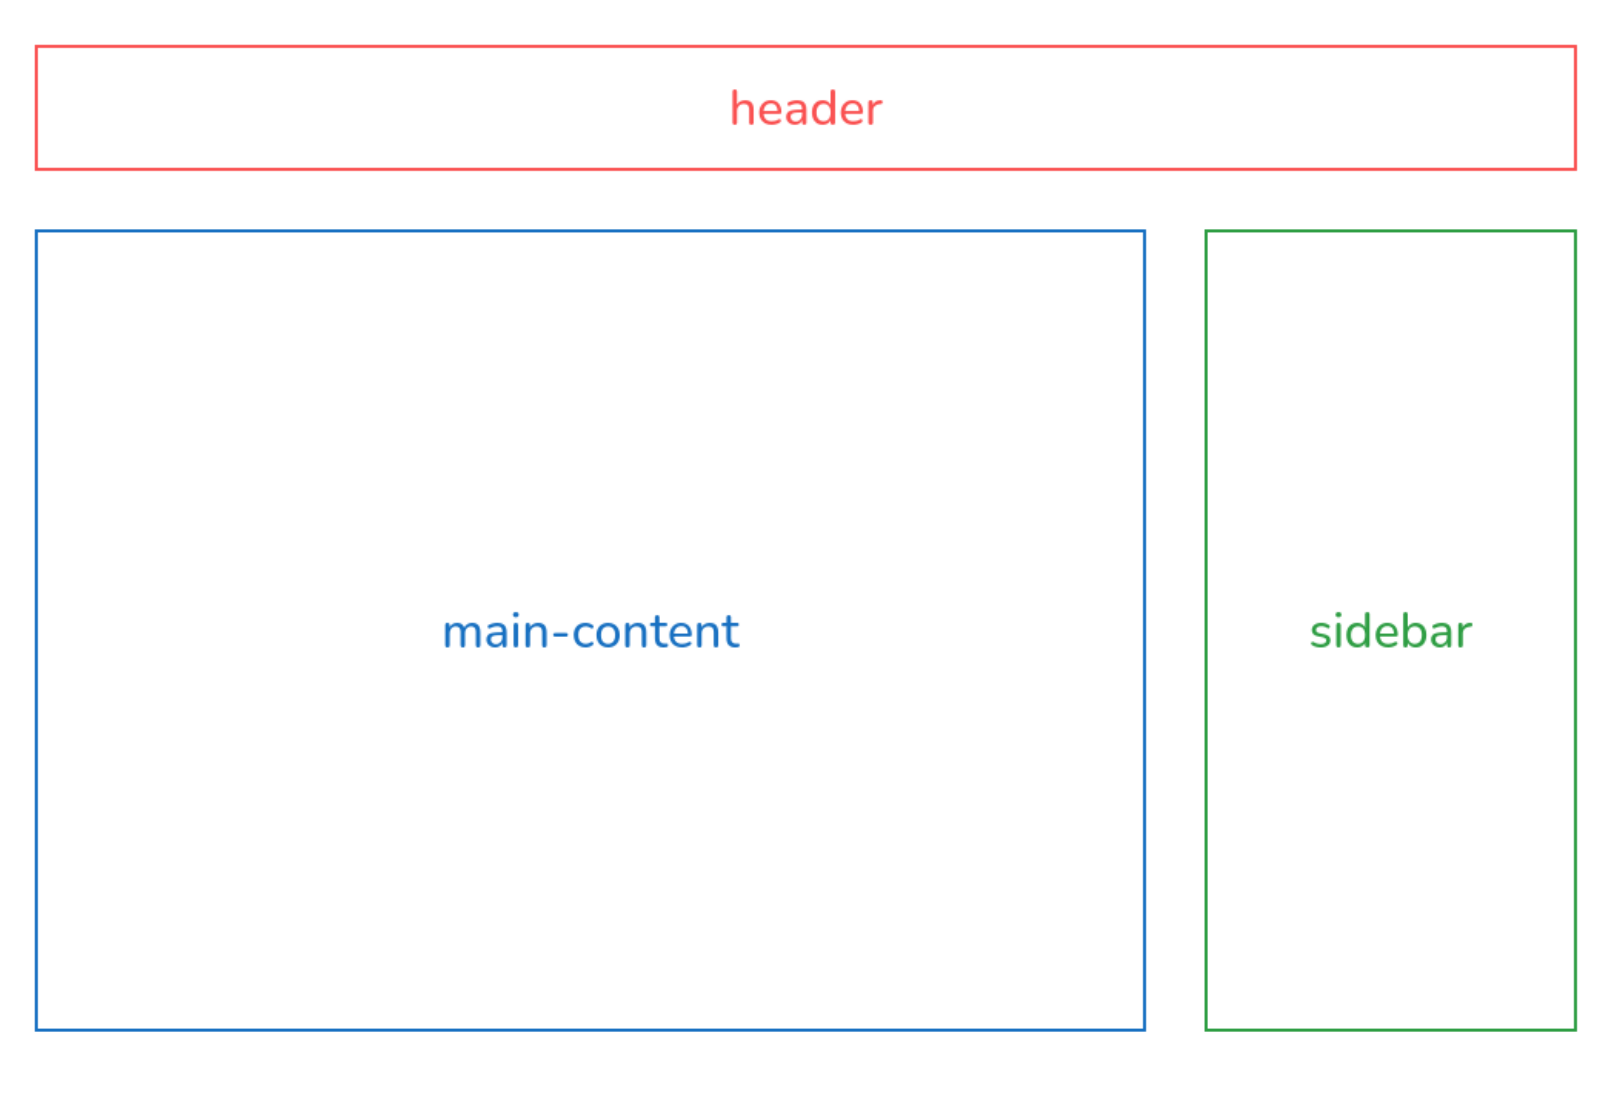
\includegraphics[width=0.9\textwidth]{gerarchia_visiva.png}
  \end{figure}
\end{frame}

\begin{frame}
  \frametitle{Tecnologie usate}

  \begin{itemize}
    \item[\faLeaf] Spring Boot
    \item[\faEnvelope] Spring Email
    \item[\faDatabase] PostgreSQL
  \end{itemize}

  \vspace{15pt}

  \begin{itemize}
    \item[\faHtml5] Angular
    \item[\faCss3] Bootstrap
  \end{itemize}

  \vspace{18pt}

  API esterne:
  \begin{itemize}
    \item[\faMapMarker] \href{https://www.openstreetmap.org/}{OpenStreetMap}
    \item[\faMapSigns] \href{https://nominatim.openstreetmap.org/}{Nominatim}
  \end{itemize}
\end{frame}

\begin{frame}
  \frametitle{Modello entità-relazione}
  \begin{figure}
    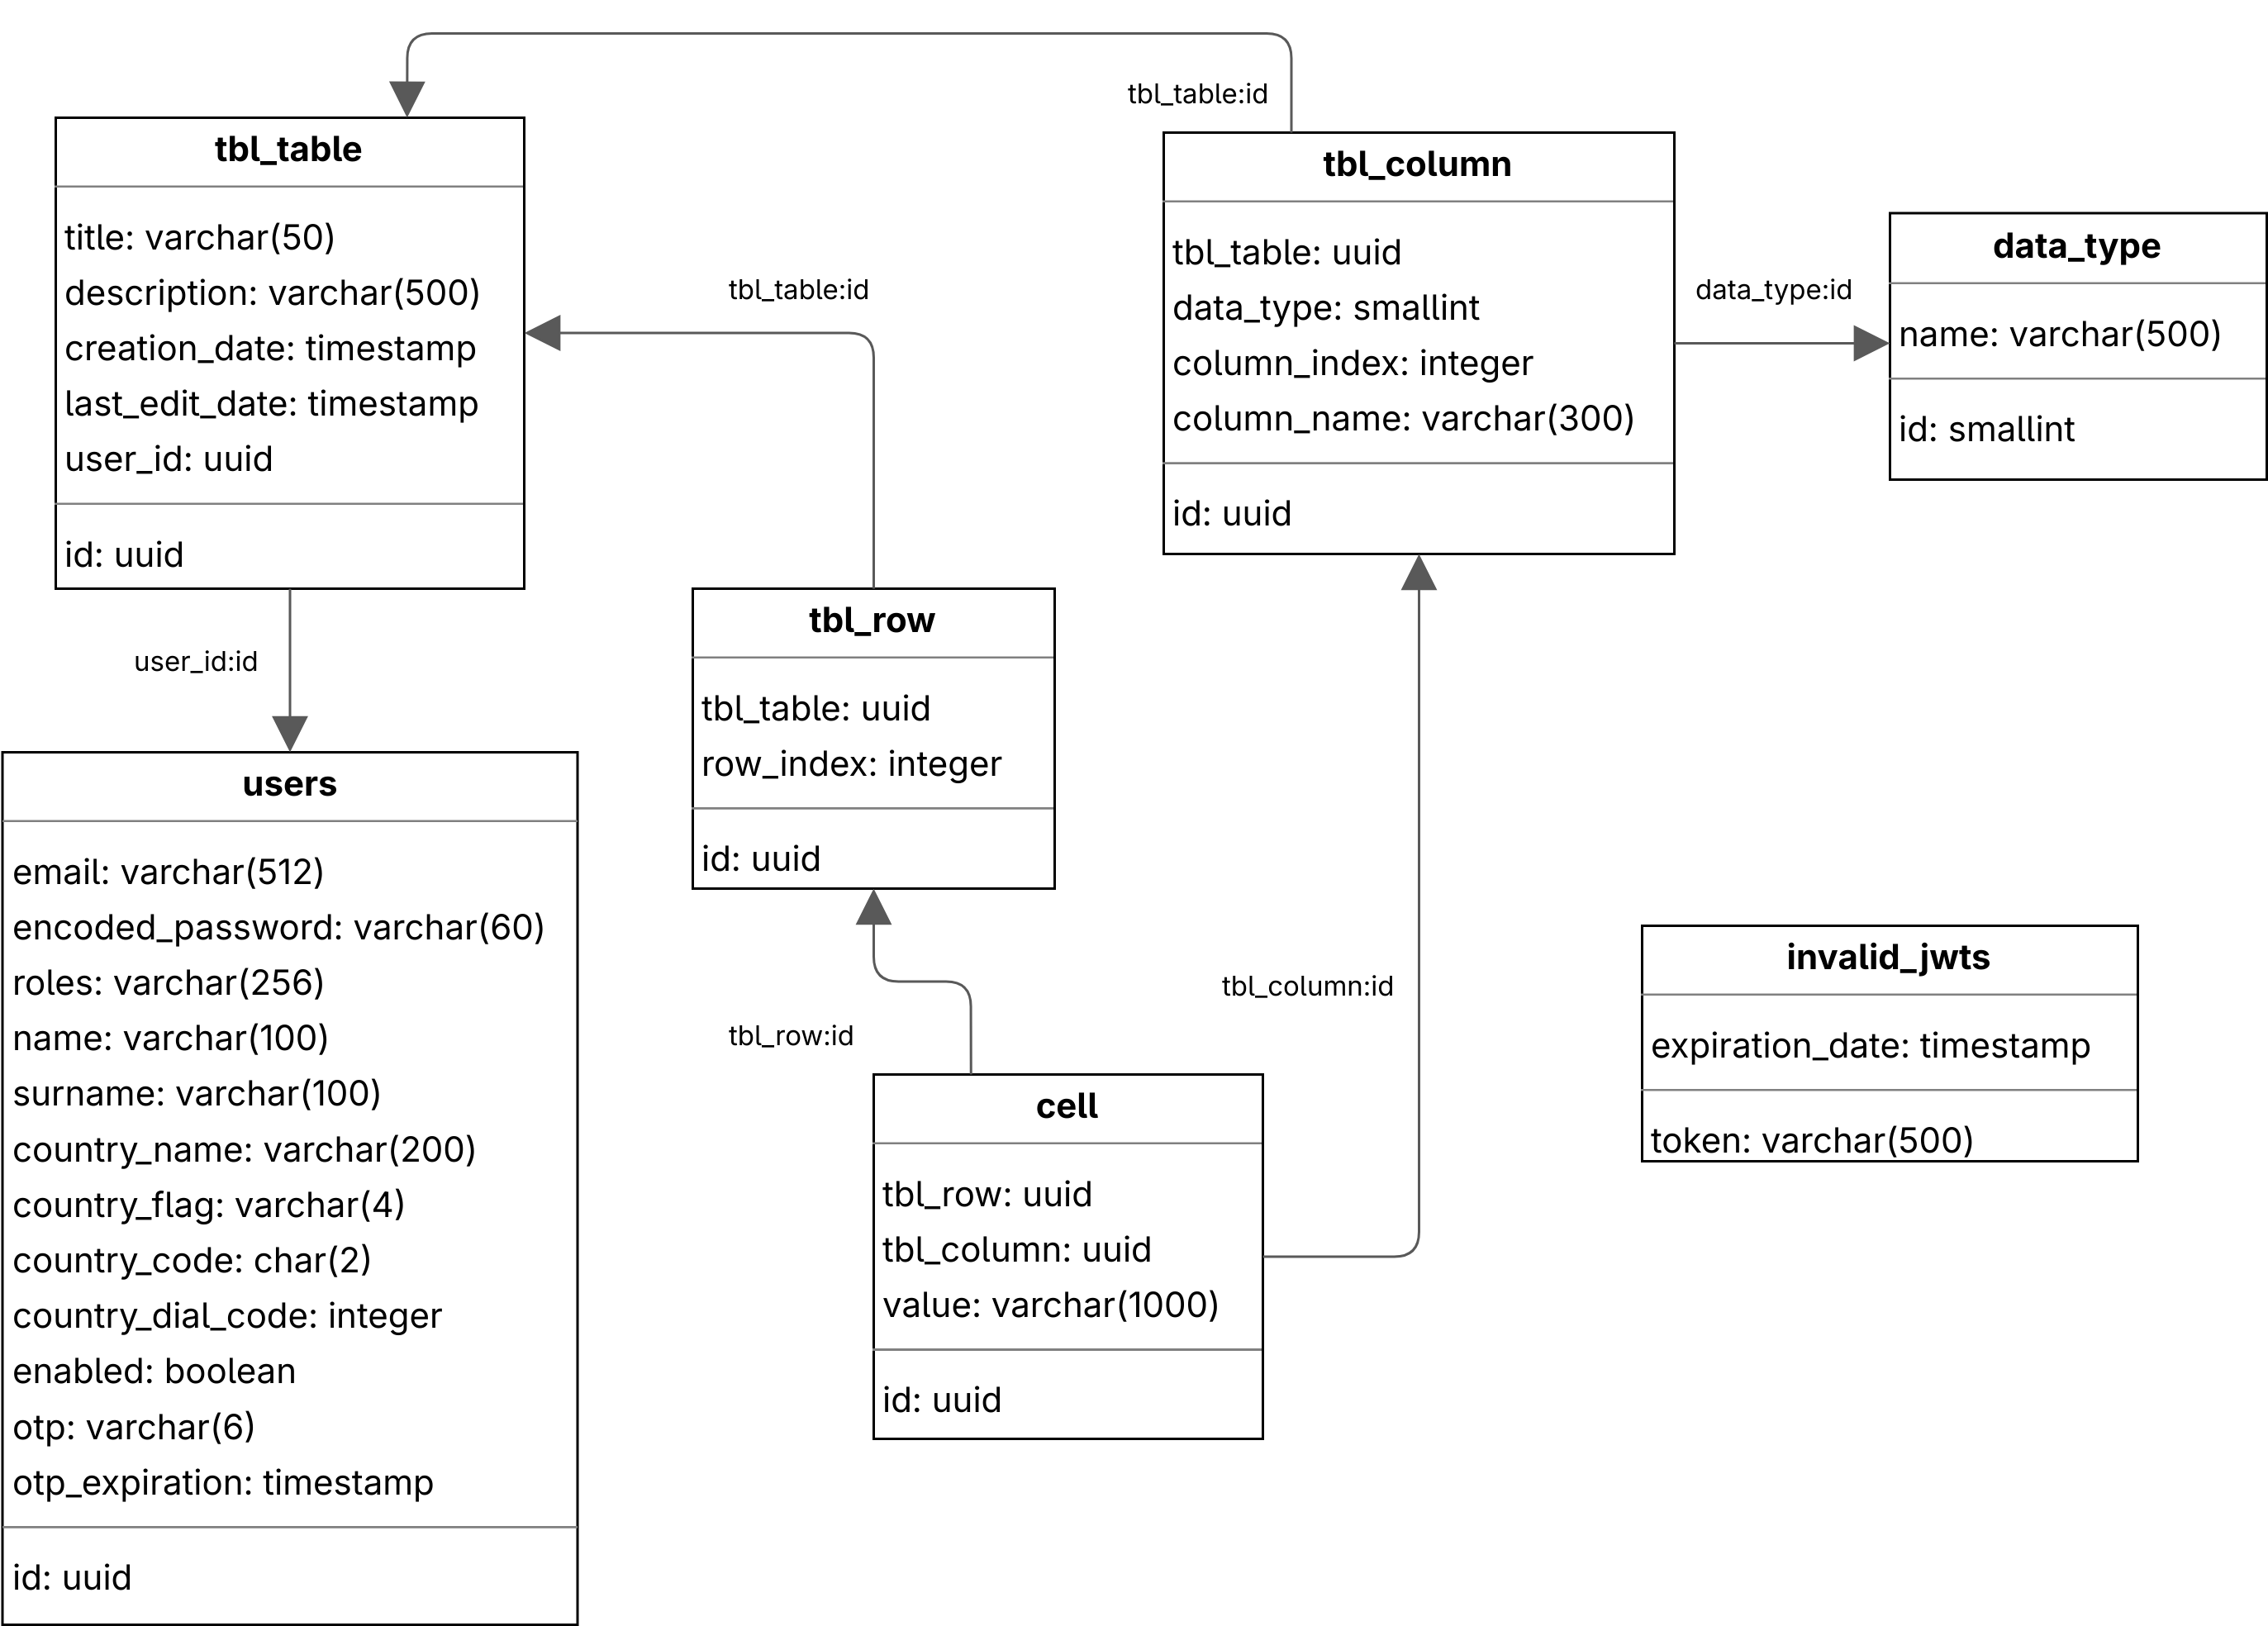
\includegraphics[width=\textwidth]{entity_relation}
  \end{figure}
\end{frame}

\begin{frame}
  \frametitle{Diagramma di classi (back-end)}
  \begin{figure}
    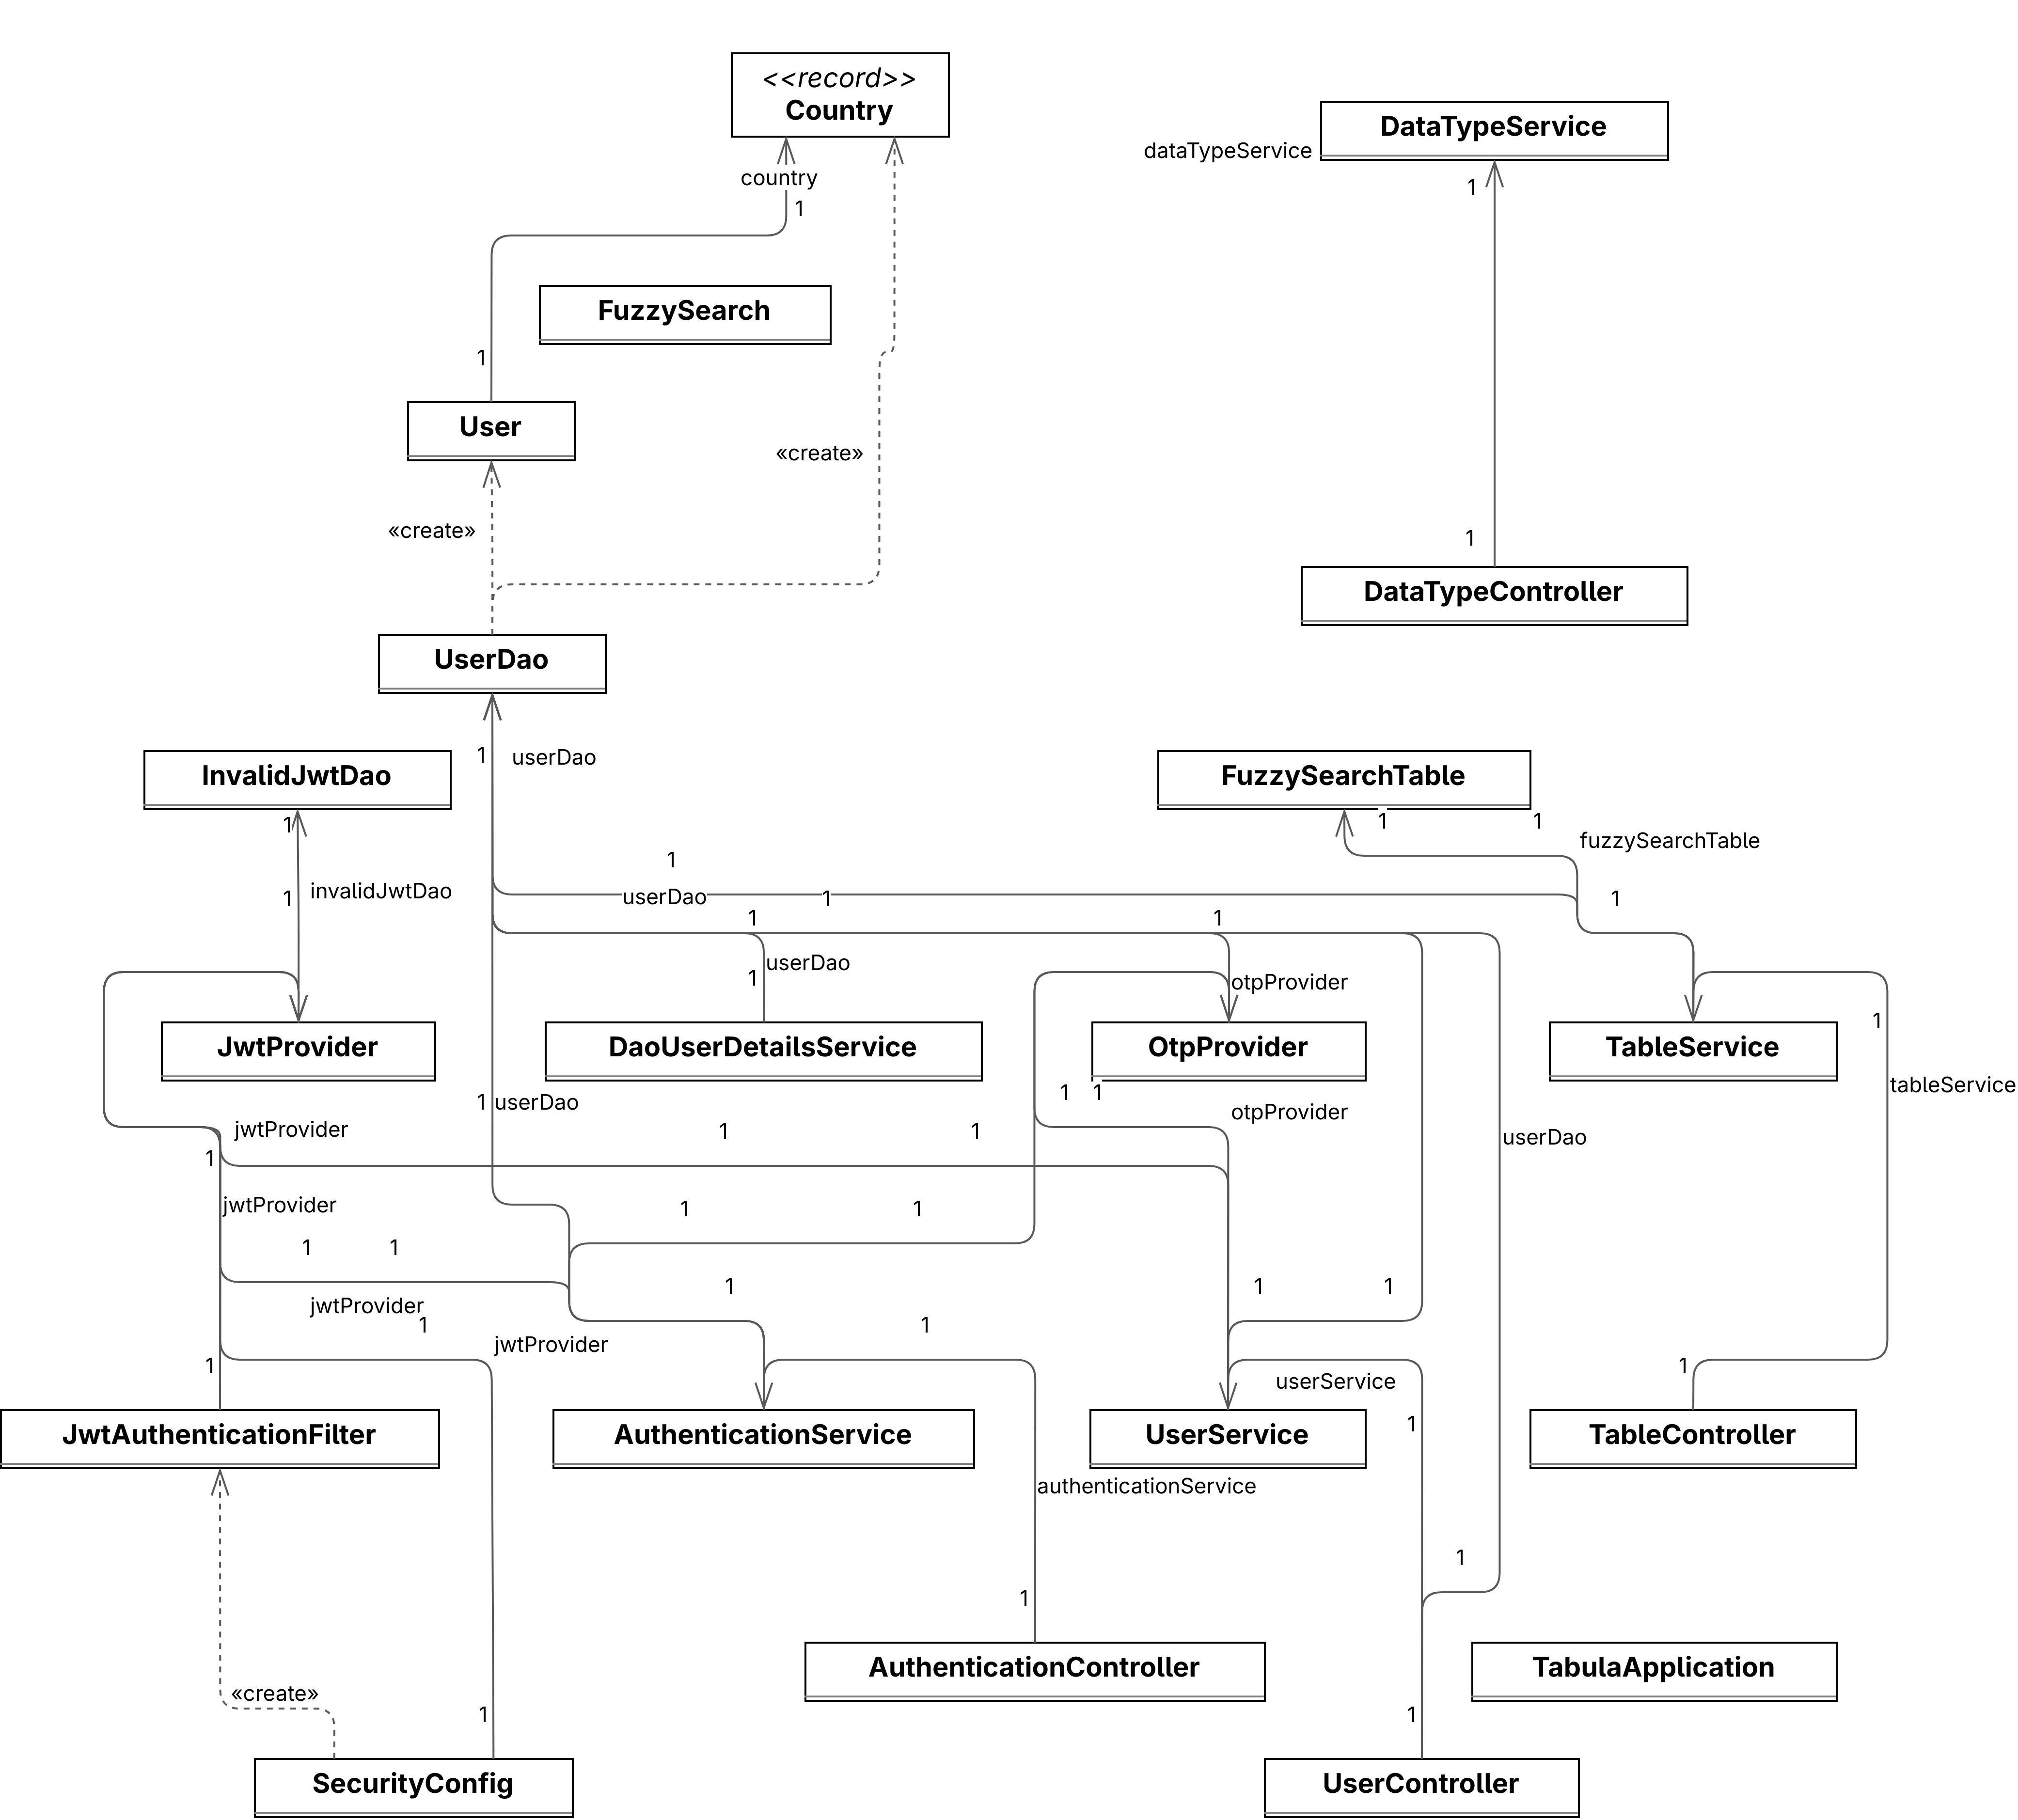
\includegraphics[height=8cm]{classes}
  \end{figure}
\end{frame}

\end{document}
